\documentclass{article}
\usepackage[utf8]{inputenc}
\usepackage[margin=1in]{geometry}

\usepackage{color}
\usepackage{amsmath}
\usepackage{amssymb}
\usepackage{caption}
\usepackage{subcaption}
\usepackage{graphicx}
\usepackage[
backend=biber,
style=ieee,
sorting=nyt
]{biblatex}
\usepackage{hyperref}

\graphicspath{ {./} }

\addbibresource{references.bib}

\title{Keeping Your Priorities Straight: \\
\large Building a Modular SDN Controller}
\author{Natalie Neamtu (nan55)}

\begin{document}

\maketitle

\section{Introduction}

With the rise of open APIs such as OpenFlow \cite{openflow} between the data plane and 
control plane, a desirable outcome would be the ability to implement 
network functionality (such as basic forwarding, access control, 
load balancing, and monitoring) using modular software components in the
control plane. Several difficulties arise in putting this idea into practice,
however, as has been documented previously (e.g., \cite{frenetic2, pyretic}). 

Consider a system composed of three modules: one that does access control,
one that load balances flows coming from external hosts, and one that does
basic shortest-paths routing.
The naive composition of these modules\textemdash simply allowing them to 
install rules on switches, as they each would when running on their own\textemdash 
has serious issues.
Firstly, the rules proposed by the access control module are likely to overlap
with those from the other modules.
To ensure that the access control policy is correctly enforced, it is important
that its rules are installed with high priority on the switches.
Secondly, the load balancing module may rely on seeing the first packet of
each flow before deciding how that flow should be routed.
If the basic routing module installs rules proactively, then it will
prevent the load balancer from seeing those packets.

In this example, we can observe that a correctly-functioning 
composition of these three modules (access control, load balancing, routing) 
will not simply act as the ``sum'' of the functionality that the modules implement
independently. 
If the access control module can be characterized as implementing
a policy such as \emph{``Drop all SSH packets from 10.0.0.1''}, 
and the load balancing module as 
\emph{``Distribute TCP flows from 10.0.0.1 to 10.0.0.99 across h2-8''}
and the routing module as 
\emph{``Route all packets on shortest paths according to destination address''}, 
then it is clear that no network can satisfy all of those policies at the same time. 
Either some packets get dropped, or all packets reach their destination.
In this case, it is evident that the access control policy should take
precedence over the load balancing policy, which should take precedence over
the routing policy. 
In general, we may take the view that whenever two such policies 
cannot be satisfied by the network simultaneously,
they should be \emph{ordered} relative to each other. 

This project focuses on composing modules in a way that abides by
this ordering. 
We refer to each module as a \emph{sub-controller}, as the interface it uses
resembles that of a typical OpenFlow controller.
Each sub-controller has a \emph{priority} which establishes to its position
in the ordering, and roughly corresponds to the numerical priority with
which that sub-controller's flow entries are installed on the switches.
The sub-controllers interface with the network devices via the
\emph{sub-controller manager}, or simply \emph{manager}, which is responsible
for installing, modifying, and deleting the flow entries on each switch, and 
ensuring that each entry is installed with the appropriate priority.
The most basic function of the manager is to install the rules requested
by the sub-controllers at the appropriate priority: such rules are called
\emph{normal} rules.
The manager also provides more sophisticated types of rules to sub-controllers: 
rules for \emph{reserving} sets of packets for installing reactive rules 
(to overcome the two-tiered programming model),
and rules for \emph{sharing} rules with other sub-controllers. 
Each of these mechanisms is explained in detail in subsequent sections. 

The rest of this report is organized as follows. 
Section \ref{ORD} describes the basics of sub-controllers, 
the sub-controller manager, and normal rules. 
Section \ref{RES} describes reservation rules, and Section \ref{SHR} describes
shared rules, including the algorithm for merging rules from different 
sub-controllers. 
Each section contains illustrating examples, whose implementations can be 
found in the source code.
Section \ref{MON} outlines how monitoring functionality could be 
added as an extension to the current system. 
Evaluation of the system is contained in Section \ref{EVA}.
Section \ref{REL} discusses related work.
This project was implemented using the POX OpenFlow library \cite{pox}.

\section{Ordered Sub-Controllers} \label{ORD}


\begin{figure}[h]
\centering
\begin{subfigure}[]{0.45\textwidth}
\centering
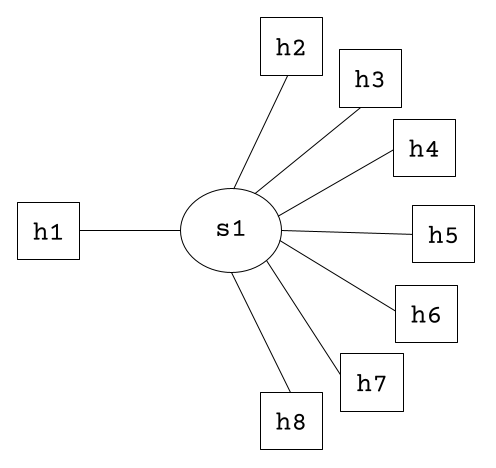
\includegraphics[width=0.85\textwidth]{topo1.png}
\caption{Eight hosts \texttt{h1-h8} connected via a single switch \texttt{s1}.
Host \texttt{hi} is connected on port \texttt{i} on \texttt{s1}.}
\label{fig:topo_1}
\end{subfigure}
\hfill
\begin{subfigure}[]{0.54\textwidth}
\centering
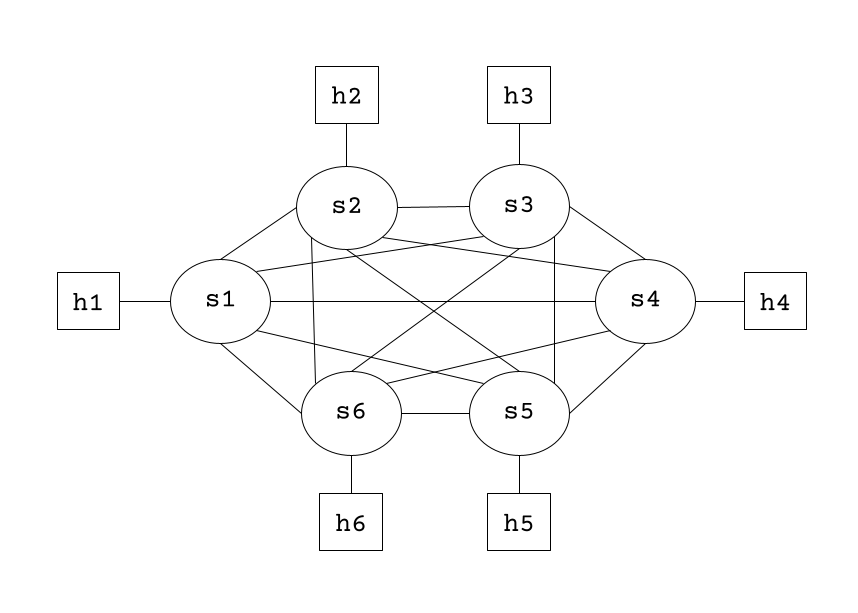
\includegraphics[width=1\textwidth]{topo2.png}
\caption{Six hosts \texttt{h1-h6} and six switches \texttt{s1-s6} 
connected in a mesh. Host \texttt{hi} is connected on port \texttt{i} to
switch \texttt{si}, and switch \texttt{sj} is connected on port \texttt{j}
to switch \texttt{si} for \texttt{i != j}.}
\label{fig:topo_2}
\end{subfigure}
\caption{Topologies used for examples.}
\label{fig:topologies}
\end{figure}

Consider the topology shown in Figure \ref{fig:topo_1}. Suppose we have
the following sub-controllers: one that implements a 
firewall for all SSH traffic from \texttt{h1} by proactively installing
rules on \texttt{s1} to drop all relevant packets, and another that
implements basic shortest-paths routing by proactively installing rules
that send packets out on the appropriate port on \texttt{s1} based on their
destination. 
Intuitively, the rules for the firewall sub-controller should be installed 
at a higher priority than those installed by the routing sub-controller.
Furthermore, if any packets are forwarded to the controller because
they did not match any of the flow entries on \texttt{s1}, they should be seen
by the firewall sub-controller before the routing sub-controller,
in case they should be dropped.

\subparagraph{Definitions.}
A \emph{match $m$} is modeled after an
OpenFlow match, and is essentially an assignment of packet header fields to
either exact values or wildcards.
To limit the scope of this project, partial/prefix matches are
not currently supported.
A \emph{packet set $ps = (m, s)$} is a match along with a switch identifier $s$. 
A packet set identifies a set of packets located at a given switch.
An \emph{action $a$} is simply an OpenFlow action
\footnote{For example, forwarding out a specified port, flooding the packet
on all ports, or rewriting a particular header field.}.
A \emph{rule} $((m, s), as)$ is a packet set with a list of actions.
A rule usually corresponds to a flow entry on an OpenFlow switch.
For now, we will discuss only \emph{normal rules} (other types of rules
will be introduced later).

\subparagraph{Sub-controllers.}
A sub-controller is a program that resembles a traditional controller
written for OpenFlow.
Each sub-controller is initialized with a unique id, and a handle for
accessing the manager's API. 
The sub-controller uses this API to tell the manager what rules it wants to 
install on the switches.
Sub-controllers must provide handlers for
each of the OpenFlow events defined by the POX library
\footnote{\url{https://noxrepo.github.io/pox-doc/html/\#openflow-events-responding-to-switches}}.
Otherwise, each sub-controller may have its own internal functions,
data structures, and state.
Sub-controllers are not allowed access to the other sub-controllers,
the rules installed by other sub-controllers, or its own priority.

\subparagraph{The sub-controller manager.}
The manager is statically configured with an ordered list of sub-controllers
$c_{0}, c_{1}, \dots, c_N$, where lower indices indicate higher priority.
As shorthand, I will write $c_{\ell} < c_h$ to indicate that $c_h$ has
higher priority than $c_{\ell}$. 
The manager also computes the priority with which each sub-controller's 
rules should be installed as a flow entry on the switches. 
We can denote the priority for $c_i$'s normal rules as $p_i^{\mathcal{N}}$. 
Given a normal rule $((m, s), as)$ from $c_i$, the manager installs an entry
with match $m$ and actions $as$ on switch $s$ with priority $p_i^{\mathcal{N}}$.
It is important that the manager ensures that if $c_{\ell} < c_h$,
then $p_{\ell}^{\mathcal{N}} < p_h^{\mathcal{N}}$.

The manager provides an API to all sub-controllers for adding, modifying,
and deleting normal rules. It also exposes the ability to send buffer
requests, giving the sub-controllers the ability to synchronize with the
switches.
The manager interfaces with all of the network devices, and thus acts as 
a middle layer between those devices and the sub-controllers.
Upon handling any of the OpenFlow events as defined by POX,
the manager calls the corresponding event handlers on each sub-controller
(described below) in order of decreasing priority. 
In the case of \texttt{PacketIn} events, sub-controllers have the option of
preventing the event from propagating to the lower priority sub-controllers
(to be used in the case when, e.g., a sub-controller has already decided
what to do with the packet).

\subparagraph{Discussion.}

Note that sub-controllers can only install normal rules at a single priority.
This is done to simplify the algorithm used to compute shared rules 
(see Section \ref{ALGO}); I have not yet explored in depth the impact on the 
algorithm of allowing sub-controllers a range of priorities for normal rules.
In addition, the current implementation of the manager simply installs 
every rule that is given to it by the sub-controllers, even if that rule 
is fully shadowed by higher-priority rules.
This is inefficient in terms of memory usage on the switches, but simple
to implement.
While I decided to leave it out of scope for this project, I believe that a
more optimized implementation is possible.

\subsection{Example A} \label{Ex_A}

Example A uses the two sub-controllers described in the paragraph opening
this section: $c_F$, the firewall sub-controller, and $c_{PR}$, 
the sub-controller that performs proactive routing. 
They are configured such that $c_F > c_{PR}$. This example uses
a topology with a single switch, like that given in Figure \ref{fig:topo_1}.

Since both $c_F$ and $c_{PR}$ are proactive, the match-action table
will be static, and will resemble that given in Table \ref{table_A}.
Here, I use the shorthand \texttt{src=hi} and \texttt{dst=hj} to denote that
the source and destination hosts of a given packet are 
\texttt{hi} and \texttt{hj}, respectively.

\begin{table}
\begin{center}
\begin{tabular}{|c|c|c|c|}
\hline
Switch & Match & Actions & Priority \\
\hline
\texttt{s1} & \texttt{src=h1} and is SSH packet & Drop & 100 \\
\hline
\texttt{s1} & \texttt{dst=h1} & Output port \texttt{1} & 0 \\
\hline
\texttt{s1} & \texttt{dst=h2} & Output port \texttt{2} & 0 \\
\hline
\dots & \dots & \dots & \dots \\
\hline
\end{tabular}
\end{center}
\caption{Representation of match-action table for Example A.}
\label{table_A}
\end{table}

\subsection{Example B} \label{Ex_B}

Example B introduces a load balancer sub-controller to the configuration in
Example A.
It uses the same topology in Figure \ref{fig:topo_1}. 
From the perspective of \texttt{h1}, TCP and UDP connections to all other 
hosts are abstracted as  coming from a single machine using a ``public'' 
IP address \texttt{10.0.0.99}.
The load balancer sub-controller $c_{LB}$ distributes TCP and UDP 
flows originating from \texttt{h1} to \texttt{h2-8} evenly. It does this by
reactively installing rules on a per-flow basis upon receiving the
first packet in an applicable flow.

Since $c_{LB}$ is reactive, the basic routing sub-controller must be made
reactive as well, as we have not yet introduced reservation rules. 
Thus, we use a reactive routing sub-controller $c_{RR}$, which also 
installs rules on a per-flow basis.

The sub-controllers are configured so that $c_F > c_{LB} > c_{RR}$.
Since $c_{LB}$ only controls the routing for a subset of flows originating
from \texttt{h1},
$c_{RR}$ is utilized when e.g., routing TCP packets between 
\texttt{h2} and \texttt{h4}.
See Table \ref{table_B} for what the match-action table on \texttt{s1} 
will look like.

\begin{table}
\begin{center}
\begin{tabular}{|c|c|c|c|}
\hline
Switch & Match & Actions & Priority \\
\hline
\texttt{s1} & \texttt{src=h1} and is SSH packet & Drop & 100 \\
\hline
\texttt{s1} & Belongs to flow \texttt{f1} & Output port \texttt{2} & 50 \\
\hline
\texttt{s1} & Belongs to flow \texttt{f2} & Output port \texttt{4} & 0 \\
\hline
\end{tabular}
\end{center}
\caption{Representation of match-action table for Example B, after
TCP flows \texttt{f1} and \texttt{f2} have been initiated, with 
\texttt{src(f1) = h1} and \texttt{dst\_ip(f1) = 10.0.0.99},
and \texttt{src(f2) = h2} and \texttt{dst(f2) = h4}.}
\label{table_B}
\end{table}

\section{Reservation Rules} \label{RES}

Example B illustrates some of the problems with composing different modules
in the two-tiered programming model that OpenFlow provides: we were forced
to make $c_{RR}$ reactive and to install rules whose matches are 
no more specific than those of $c_{LB}$. In this section, we describe
\emph{reservation rules}, which are an attempt to resolve these issues.

A reservation rule is simply a packet set, as no actions specified
by the sub-controller are required. 
By adding a reservation rule for a packet set $(m, s)$, a sub-controller 
$c_i$ is able to prevent the corresponding packets from falling under the 
control of the rules installed by lower priority sub-controllers $c_j < c_i$.
More specifically, the sub-controller manager will install a flow entry 
on switch $s$ with match $m$ and actions directing the switch to 
forward corresponding packets to the controller.
This flow entry will have priority $p_i^{\mathcal{R}}$ such that
$p_i^{\mathcal{R}} < p_i^{\mathcal{N}}$ and 
$p_j^{\mathcal{N}} < p_i^{\mathcal{R}}$ for all $j$ such that $c_j < c_i$.
That is, a reservation rule will not interfere with $c_i$'s
normal rules, but it will preempt the rules of the lower priority sub-controllers.
Upon receiving a packet as a result of a reservation rule, 
the manager will first pass the packet to the highest priority sub-controller 
whose reservations encompass that packet.
As is the case with \texttt{PacketIn} events, sub-controllers
can choose whether to allow this event to propagate to lower-priority
sub-controllers.
The manager provides an API to the sub-controller for adding or removing 
reservations. Each sub-controller must provide a handler for when
reserved packets are received by the manager.

The model that should be adopted is that if $c_i$ wishes to install 
reactive rules for some packet set, it must install a reservation rule for that
packet set. 
It is not safe in general to assume that lower priority 
sub-controllers will not install rules overlapping that packet set.
This model allows easier reuse and reordering of sub-controllers without
losing the desired functionality.

\subsection{Example C} \label{Ex_C}

Example C illustrates how reservations enable the composition of a 
proactive basic routing strategy with a reactive routing strategy on
a subset of flows. It uses the topology given in Figure \ref{fig:topo_2}.
In this example, we compose the routing sub-controller $c_{PR}$
with a sub-controller $c_{VLB}$ that implements a reactive version of
Valiant Load-Balancing on TCP traffic on a per-flow basis.

For each new TCP flow, $c_{VLB}$ chooses a second hop by going round-robin
for each source host. It then installs the entries for that
flow on the appropriate switches. Since $c_{PR}$ is proactive, 
$c_{VLB}$ must add reservation rules for all TCP packets.
At the same time, $c_{PR}$ can be indifferent to the strategy adopted
by $c_{VLB}$, and install proactive rules at whatever granularity it wishes.
A representation of the match-action tables after a single TCP flow has
been started is given in Table \ref{table_C}.

\begin{table}
\begin{center}
\begin{tabular}{|c|c|c|c|}
\hline
Switch & Match & Actions & Priority \\
\hline
\texttt{s1} & Belongs to flow \texttt{f1} & Output port \texttt{3} & 100 \\
\hline
\texttt{s3} & Belongs to flow \texttt{f1} & Output port \texttt{2} & 100 \\
\hline
\texttt{s2} & Belongs to flow \texttt{f1} & Output port \texttt{2} & 100 \\
\hline
\texttt{s1-s6} & Is TCP packet & Send to controller & 99 \\
\hline
\texttt{s1-s6} & \texttt{dst=h1} & Output port \texttt{1} & 0 \\
\hline
\texttt{s1-s6} & \texttt{dst=h2} & Output port \texttt{2} & 0 \\
\hline
\dots & \dots & \dots & \dots \\
\hline
\end{tabular}
\end{center}
\caption{Representation of match-action table for Example C, after
TCP flow \texttt{f1} has been initiated, with \texttt{src(f1) = h1} and
\texttt{dst(f1) = h2}.}
\label{table_C}
\end{table}

\section{Shared Rules} \label{SHR}

So far, we have been dealing with situations where the flow entries installed
by one sub-controller should preempt and replace those installed by another
sub-controller. This is not flexible enough for all applications, as 
there are many instances where the flow entries should be ``merged'' in 
some way. For example, we may wish to combine a monitoring sub-controller
with a shortest-path routing sub-controller. 
The monitoring functionality should not get in the way of the 
routing functionality, and vice versa.
This section describes this project's method for doing such composition:
\emph{shared rules}.

Unlike with normal and reservation rules, when a sub-controller adds rules of this 
new type, they may not correspond exactly to the flow entries that are
installed on the switch, due to the merging algorithm. 
Thus, we must distinguish between \emph{sharable rules},
which are specified by the sub-controller, and \emph{shared rules},
which are computed by the sub-controller manager by applying 
the merging algorithm to each sharable rule.
Each sharable rule can correspond to multiple shared rules.

A sharable rule is a packet set and an optional list of actions.
Roughly speaking, a sub-controller $c_i$ can add a 
sharable rule $(ps, as)$ if it wishes to allow
lower priority sub-controller to execute actions on packets
that belong to $ps$. 
If $c_j < c_i$ adds a normal or sharable rule $(ps', as')$ such
that $ps$ \emph{overlaps} with $ps'$, then the manager will compute a new
rule which applies the actions $as$, followed by the actions $as'$, 
to all packets in the \emph{intersection} of $ps$ and $ps'$.
Once a sharable rule is converted to a set of shared rules, they will 
be installed as flow entries on switches with a priority higher 
than $p_i^{\mathcal{N}}$
(however, this priority can vary across the shared rules 
for $c_i$, as described below).
Therefore, by adding a sharable rule $(ps, \texttt{[]})$ with no actions specified,
$c_i$ can also allow the rules from lower priority sub-controllers to preempt 
its own normal rules over the packet set $ps$.

The manager provides an API to add, modify, and remove sharable rules.
Modifying or removing a sharable rule will change all shared rules that 
are derived from that sharable rule.

\subsection{Merging Algorithm} \label{ALGO}

The merging algorithm can be characterized as follows: beginning with the
sharable rules for some sub-controller $c_i$, it first merges with the
normal and sharable rules for $c_{i+1}$ 
(the sub-controller with the next-lowest priority). 
This merging is done on a per-rule basis.
When merging sharable rule $(ps, as)$ from $c_i$ with $(ps', as')$ with
$c_{i+1}$, the algorithm should ensure:
\begin{itemize}
\item[(1)] If $ps$ overlaps with $ps'$, then the resulting set of rules
should ensure that all packets in the intersection of $ps$ and $ps'$ are
processed first using the actions $as$, followed by the actions $as'$;
\item[(2)] If $as$ is non-empty, then the resulting set of rules
should ensure that all packets in $ps$ (but not in $ps'$) are processed using 
the actions $as$;  
\item[(3)] If $(ps', as')$ is sharable, then any rules created to 
satisfying (1) should also be sharable 
with the remaining sub-controllers $c_{i+2}, \dots, c_{N}$.
Otherwise, the resulting rules should not be sharable with the remaining
sub-controllers.
Note that any rules resulting from satisfying (2) will be sharable, since
$(ps, as)$ is sharable.
\end{itemize}
(1) and (2) ensure that $c_i$'s actions still get carried out on all
packets in $ps$. (1) allows $c_{i+1}$'s actions to be applied to 
a subset of packets in $ps'$, as allowed by the sharable rule.
(3) means that sharable rules ``trickle-down'', so that if successive
sub-controllers provide sharable rules overlapping with $ps$ and $ps'$, 
the sub-controller with the next-lowest priority can merge its rules for 
that packet set.
Note that (1) and (2) require that the algorithm produce rules of differing
priorities.

After processing $c_{i+1}$'s rules,
the algorithm recurses on the next sub-controller's rules.
Note that for each rule that the algorithm outputs, we can ``trace''
which sub-controllers had their rules merged to create that shared rule.
Thus, in order to abide by the relative priorities of the sub-controllers, 
the algorithm must also ensure:
\begin{itemize}
\item[(4)] For any $c_j, c_k$ such that $c_k < c_j < c_i$, 
the rules resulting from merging with $c_j$'s rules (i.e. to satisfy (1)) 
must have a higher priority than the rules resulting from merging 
with $c_k$'s rules only (i.e., not both $c_j$ and $c_k$'s rules).
\end{itemize}

\begin{figure}
\centering
\begin{subfigure}{1.0\textwidth}
\begin{center}
\begin{tabular}{|c|c|c|}
\hline
Sub-controller & Rule & Type \\
\hline
$c_h$ & $\texttt{((ip\_src=10.0.0.1 \& ip\_dst=10.0.0.2, s1), ah)}$ & Sharable \\
\hline
$c_m$ & $\texttt{((ip\_src=10.0.0.1, s1), am)}$ & Normal/Sharable \\
\hline
$c_{\ell}$ & $\texttt{((ip\_dst=10.0.0.2 \& in\_port=0, s1), al)}$ & Normal \\
\hline
\end{tabular}
\end{center}
\caption{Rules for each sub-controller.}
\label{table_algo_a}
\end{subfigure}
\par\bigskip
\begin{subfigure}{1.0\textwidth}
\begin{center}
\begin{tabular}{|c|c|c|}
\hline
& Shared Rule &  \\
\hline
$\texttt{r1}$ & $\texttt{((ip\_src=10.0.0.1 \& ip\_dst=10.0.0.2, s1), ah + am)}$
& $c_h, c_m$ \\
\hline
$\texttt{r2}$ & $\texttt{((ip\_src=10.0.0.1 \& ip\_dst=10.0.0.2 \& in\_port=0, s1), ah + al)}$
& $c_h, c_{\ell}$ \\
\hline
\end{tabular}
\end{center}
\caption{When $c_m$'s rule is a normal rule. 
Rules listed in order of decreasing priority. 
Corresponding sub-controllers are in the rightmost column.}
\label{table_algo_b}
\end{subfigure}
\par\bigskip
\begin{subfigure}{1.0\textwidth}
\begin{center}
\begin{tabular}{|c|c|c|}
\hline
& Shared Rule & \\
\hline
$\texttt{r0}$ & $\texttt{((ip\_src=10.0.0.1 \& ip\_dst=10.0.0.2 \& in\_port=0, s1), ah + am + al)}$
& $c_h, c_m, c_{\ell}$ \\
\hline
$\texttt{r1}$ & $\texttt{((ip\_src=10.0.0.1 \& ip\_dst=10.0.0.2, s1), ah + am)}$
& $c_h, c_m$ \\
\hline
$\texttt{r2}$ & $\texttt{((ip\_src=10.0.0.1 \& ip\_dst=10.0.0.2 \& in\_port=0, s1), ah + al)}$
& $c_h, c_{\ell}$ \\
\hline
\end{tabular}
\end{center}
\caption{When $c_m$'s rule is a sharable rule.
Rules listed in order of decreasing priority. 
Corresponding sub-controllers are in the rightmost column.}
\label{table_algo_c}
\end{subfigure}
\caption{Example results of merging algorithm for sub-controllers $c_{\ell} < c_m < c_h$.}
\label{table_algo}
\end{figure}

\subparagraph{Example.} 
Suppose we have 3 sub-controllers $c_{\ell} < c_m < c_h$ which have the
rules given in Figure \ref{table_algo_a}. 
We begin with the scenario where $c_m$'s rule is a normal rule.
Merging $c_h$ and $c_m$'s rules produces shared rule $\texttt{r1}$ in 
Figure \ref{table_algo_b}.
Since $c_m$'s rule is not sharable, $\texttt{r1}$ should not be sharable
with $c_{\ell}$.
Thus, we will only merge $c_h$ and $c_{\ell}$'s rules, and this produces
$\texttt{r2}$. 
Note that, because of (4),
$\texttt{r2}$ should have a lower priority than $\texttt{r1}$. 
In this scenario, the packet sets for $\texttt{r1}$
and $\texttt{r2}$ are equivalent, so $\texttt{r2}$ will not be applied to 
any packets. However, the algorithm will still compute $\texttt{r2}$, and
the manager will install the corresponding flow entry on the switch.
This is done only in order to simplify 
the case where $c_m$ deletes its rule: we only need to remove $\texttt{r1}$
from the switch, as $\texttt{r2}$ is already installed.

If $c_m$'s rule is instead sharable, then we would need to compute a third
shared rule, which is the result of merging $\texttt{r1}$ and $c_{\ell}$'s
rule. This is $\texttt{r0}$, as depicted in Figure \ref{table_algo_c}.
Due to (1) and (2), $\texttt{r0}$ has the highest priority out of all three
shared rules. 

\subparagraph{Algorithm details.}

First, we introduce some definitions. 
A packet set $ps$ can be thought of as matching a set of packets
(i.e. packets with particular header entries, and located at a particular
switch).
Given packet sets $ps$ and $ps'$, let $ps \cap ps'$ denote the packet set 
that matches all packets matched by both $ps$ and $ps'$.
And given two lists of actions $as$ and $as'$, let $as + as'$ denote the
concatenation of $as$ and $as'$.

For the purposes of the merging algorithm, each rule is now a 4-tuple
$(ps, as, p, b)$, where $ps$ is a packet set, $as$ is a list of actions, 
$p$ is a symbolic priority, and $b$ is a boolean value indicating whether
the rule is sharable or not.
A \emph{symbolic priority} is a list of natural numbers.
Symbolic priorities are ordered according to their head element;
see Figure \ref{fig:symbolic_priorities}. 
As is explained below, symbolic priorities help
us keep track of which sub-controllers' rules were merged
to create a given rule. 
Each sub-controller $c_i$ maps to a natural number $n(c_i) = N-i$ 
which represents its priority numerically, so that if $c_i > c_j$,
then $n(c_i) > n(c_j)$.

\setlength{\tabcolsep}{2pt}
\begin{figure}
\centering
\begin{tabular}{l l l}
  
  \begin{tabular}{r l}
    $n ::=$ & $\mathbb{N}$ \\

    $p ::=$ & $\texttt{[]} ~|~ n :: p$
  \end{tabular}
& \hskip 14pt
  \begin{tabular}{r l}
    \texttt{[]} =& \texttt{[]} \\
    $n :: p$ =& $n' :: p' \text{ ~if } p = p' \text{ \& } n = n'$
  \end{tabular}
& \hskip 14pt
  \begin{tabular}{r l}
    \texttt{[]} $<$&$n :: p$ \\
    $\ell :: p <$ &$h :: p' \text{ ~if } \ell < h$ \\
    $n :: p <$&$n :: p' \text{ ~if } p < p'$ \\
  \end{tabular}
  
\end{tabular}
\caption{Symbolic priorities: BNF, equality, and ordering.}
\label{fig:symbolic_priorities}
\end{figure}
\setlength{\tabcolsep}{6pt}

For each sub-controller $c_i$, define $N_{i}, H_{i}$ as the following: 
$$N_{i} = \{(ps, as, n(c_i) :: \texttt{[]}, \texttt{FALSE}) ~|~ c_{i}\text{ has normal rule } (ps, as)\}$$
$$H_{i} = \{ (ps, as, n(c_i) :: \texttt{[]}, \texttt{TRUE}) ~|~ c_{i}\text{ has sharable rule } (ps, as) \}$$

The merging algorithm works as follows.
Beginning with the sharable rules for $c_h$, and letting $S_h = H_h$,
we first merge with the normal and sharable rules for $c_{h+1}$. 
This results in a new set of rules, denoted $S_{h+1}$.
The process is then repeated recursively on $S_{h+2}$ and $c_{h+2}$'s rules,
and so on, until we have merged with $c_N$'s rules to produce $S_N$. 
The set of rules $S_N$ become the shared rules that are installed as flow
entries on the switches.

Here, I will describe the process to compute $S_{i+1}$ from $S_i$ and 
$c_{i+1}$'s rules. 
Iterating over each rule $(ps, as, p, b) \in S_i$ and 
each rule $(ps', as', p', b') \in N_{i+1} \cup H_{i+1}$, 
we compute a set of rules $R$ as follows:
\begin{itemize}
  \item If $b = \texttt{FALSE}$, then \textbf{continue};
  \item Otherwise, if $b = \texttt{TRUE}$, then:
  \begin{itemize}
    \item If $ps~ \cap ~ps'$ is non-empty, then 
    $R := R \cup \{(ps \cap ps', as + as', \texttt{concat}(p, p'), b')\}$;
    \item Otherwise, \textbf{continue}.
  \end{itemize} 
\end{itemize}

Finally, we set $S_{i+1}$ to be the union $S_{i+1} = S_i \cup R$.

To convert $S_N$ to a set of shared rules to be installed on the switches,
we need to convert the symbolic priority to a numerical priority, 
while also preserving the ordering relation. 
This can be done by first popping the head $n(h)$ off each priority $n(h)::p$
(since all priorities have $n(h)$ as the head, it is not necessary to preserve
the ordering). 
Then, we can do the conversion as follows:
\begin{align*}
  \texttt{num}(\texttt{[]}) &= 0 \\
  \texttt{num}(n :: p) &= 2^n + \texttt{num}(p)
\end{align*}

Finally, each rule's priority must be offset by adding $p_h^{\mathcal{N}} + 1$.
The result is that the shared rules for $c_h$ span the range of priorities 
from $p_h^{\mathcal{N}} + 1$ to $p_h^{\mathcal{N}} + 1 + (2^{n(h)} - 1)$ on the switches.


\subparagraph{Discussion.}

There are some inefficiencies present in the current implementation of 
the merging algorithm. As mentioned above, the manager will
sometimes install a flow entry that will never be used, given the
current configuration of the match-action table.
As these tables have finite memories, this is not ideal.
The number of shared rules installed on the switch is, in the worst case,
exponential in the number of original sharable rules.
For the purposes of this project, exploring any optimizations relating
to this issue were considered out of scope.
The authors of PANE \cite{participatory_networking} found an optimization for
their conflict resolution algorithm that suffered from a similar issue,
and they reduced their space complexity to $O(n^2)$.

It is also worth mentioning that in the current version of the algorithm,
the shared rules can be computed fully on a per-rule basis. That is,
adding or deleting a rule (whether by the sub-controller $c_h$ whose
shared rules are being computed, or by a lower priority sub-controller)
will only affect the shared rules derived from that rule. 
None of the other rules need to be recomputed by the manager,
or changed on the switches.
This greatly simplifies the problem of making shared rules dynamic, as 
it is easy to handle sub-controllers modifying rules on the fly.

Another significant inefficiency of this algorithm is the large
range of priorities it requires from the switch. This range
grows exponentially in the number of sub-controllers. 
Thus, the number of possible sub-controllers on an OpenFlow switch with
$2^{16}=$65,536 possible priorities is just 14 (recall that we need a couple priorities
for normal and reservation rules). 
Again, this comes with the trade-off of a scheme that is simple to make dynamic.
For this project, I opted to go with the simpler scheme, as it is still
able to scale with all of the examples included in this report.

A possible alternative would be to simply sort the symbolic priorities
$p_0 < \dots < p_m$ of the shared rules, and assign a numerical priority
of $0, \dots, m$ (plus the appropriate offset $p_h^{\mathcal{N}} + 1$) accordingly.
With this scheme, however, we can no longer depend on the fact that
adding or removing shared rules will not affect other shared rules.
For instance, adding a shared rule may cause the priorities of other
shared rules to increase. This makes handling the adding and removing
of shared rules more complicated, as many flow entries may need to be changed.
Further, as statistics are collected for each flow entry on the switches,
this means that the manager would have to become more involved in 
performing monitoring, as it would have to mask these changes in flow
entries from the sub-controllers.

Finally, the merging algorithm does not handle OpenFlow actions that modify 
header fields well. There are two cases to consider.
The first case is when we would like to do sequential composition (in the
style of NetKAT \cite{netkat} or Pyretic \cite{pyretic}), where a 
rewrite in a higher priority sub-controller's actions would ideally trigger
a match on a \emph{different} packet set in the lower priority sub-controller's
rules.
The second case is when we would like to do parallel composition (e.g., as in
Frenetic \cite{frenetic1}), where a rewrite in a higher priority 
sub-controller's actions causes a modified version of the packet to be sent out
due to the lower priority sub-controller's actions (as the rewrite is never 
undone).
Thus, the current version of the algorithm is only well-suited to actions
that send the packet out particular port(s).

\subsection{Example D} \label{Ex_D}

Example D illustrates how sharable rules can be used to allow a sub-controller
to effectively construct a ``set difference'' for the packet sets it uses
for its rules. 
This example uses the VLB controller $c_{VLB}$ from Example C
and the proactive routing sub-controller $c_{PR}$.
This time, $c_{VLB}$ is configured to add a sharable rule for SSH traffic with
no corresponding actions. The result is that $c_{PR}$'s actions are 
able to be applied to SSH traffic, so these packets are routed on shortest paths.
A representation of what the match-action tables will look like is given in 
Table \ref{table_D}.

\begin{table}
\begin{center}
\begin{tabular}{|c|c|c|c|c|}
\hline
Switch & Match & Actions & Priority & Type \\
\hline
\texttt{s1-6} & \texttt{dst=h1} and is SSH packet & Output port \texttt{1} & 6 & Shared \\
\hline
\texttt{s1-6} & \texttt{dst=h2} and is SSH packet & Output port \texttt{2} & 6 & Shared \\
\hline
\dots & \dots & \dots & \dots & \dots \\
\hline
\texttt{s1} & Belongs to flow \texttt{f1} & Output port \texttt{3} & 4 & Normal \\
\hline
\texttt{s3} & Belongs to flow \texttt{f1} & Output port \texttt{2} & 4 & Normal \\
\hline
\texttt{s2} & Belongs to flow \texttt{f1} & Output port \texttt{2} & 4 & Normal \\
\hline
\texttt{s1} & Is TCP packet & Send to controller & 3 & Reservation \\
\hline
\texttt{s1-6} & \texttt{dst=h1} & Output port \texttt{1} & 1 & Normal \\
\hline
\texttt{s1-6} & \texttt{dst=h2} & Output port \texttt{2} & 1 & Normal\\
\hline
\dots & \dots & \dots & \dots & \dots \\
\hline
\end{tabular}
\end{center}
\caption{Representation of match-action table for Example D, after
TCP flow \texttt{f1} has been initiated, with \texttt{src(f1) = h1} and
\texttt{dst(f1) = h2}.}
\label{table_D}
\end{table}

\subsection{Example E} \label{Ex_E}

Example E demonstrates how shared rules can enable multiple sub-controller
to implement their ``polices'' in parallel. It introduces a new
sub-controller, $c_{EO}$, which is called an ``even-host observer''.
The job of $c_{EO}$ is to ensure that packets from all hosts \texttt{hi} 
that are numbered with an even number \texttt{i} are sent to the controller
(i.e., ``observed''). However, this monitoring should not interfere with
the normal routing in the network.
Thus, for each even host \texttt{hi}, $c_{EO}$ adds a sharable rule
$\texttt{((src=hi, si), CONTROLLER)}$ to switch \texttt{si}.

When $c_{EO}$ is configured with $c_{PR}$ such that $c_{EO} > c_{PR}$,
the match action tables on the switches will resemble that in
Table \ref{table_E}. 
The rules shown are for the topology in Figure \ref{fig:topo_2}.

\begin{table}
\begin{center}
\begin{tabular}{|c|c|c|c|c|}
\hline
Switch & Match & Actions & Priority & Type \\
\hline
\texttt{s2} & \texttt{src=h2 \& dst=h1} & Send to Controller, Output port \texttt{1} & 6 & Shared \\
\hline
\texttt{s2} & \texttt{src=h2 \& dst=h2} & Send to Controller, Output port \texttt{2} & 6 & Shared \\
\hline
\dots & \dots & \dots & \dots & \dots \\
\hline
\texttt{s4} & \texttt{src=h4 \& dst=h1} & Send to Controller, Output port \texttt{1} & 6 & Shared \\
\hline
\texttt{s4} & \texttt{src=h4 \& dst=h2} & Send to Controller, Output port \texttt{2} & 6 & Shared \\
\hline
\dots & \dots & \dots & \dots & \dots \\
\hline
\texttt{s6} & \texttt{src=h6 \& dst=h1} & Send to Controller, Output port \texttt{1} & 6 & Shared \\
\hline
\texttt{s6} & \texttt{src=h6 \& dst=h2} & Send to Controller, Output port \texttt{2} & 6 & Shared \\
\hline
\dots & \dots & \dots & \dots & \dots \\
\hline
\texttt{s1-6} & \texttt{dst=h1} & Output port \texttt{1} & 1 & Normal \\
\hline
\texttt{s1-6} & \texttt{dst=h2} & Output port \texttt{2} & 1 & Normal\\
\hline
\dots & \dots & \dots & \dots & \dots \\
\hline
\end{tabular}
\end{center}
\caption{Representation of match-action table for Example E.}
\label{table_E}
\end{table}

\section{Monitoring: Outline} \label{MON}

In this section, I will describe how simple monitoring functionality could
be implemented using shared rules. 
Unfortunately, I ran out of time to implement this before the deadline.
However, I still wanted to include the idea, since the design of the shared rules
was influenced by the hope that they could be used for monitoring.

The idea is that the monitoring that a sub-controller $c_i$ wants to perform
will be instrumented using a separate sub-controller, $m_{c_i}$. 
Typically, $m_{c_i}$ would have a higher priority than $c_i$.
A typical configuration might be to prioritize all monitoring sub-controllers 
so that they occupy the highest priority slots in the whole system.
Monitoring sub-controllers $m_{c_i}$ will provide two types of \emph{monitoring}
rules to $c_i$:
one that \emph{counts} packets in a packet set, and another that \emph{observes}
all packets in a packet set by sending them to the subscribed sub-controller
(the choice for these operations was inspired by Pyretic).
Rather than communicating directly with the manager, $c_i$ will add, modify,
and delete its monitoring rules via $m_{c_i}$'s API. 
In turn, $m_{c_i}$ will communicate those rules to the manager, as follows:
\begin{itemize}
\item For count rules on packet set $ps$, $m_{c_i}$ adds a sharable rule for
$ps$ with no specified actions. This ensures that any processing added
by lower priority sub-controllers on some subset of $ps$ will be done using
rules that match \emph{only} packets in $ps$. 
If no shared rule is computed that matches all of $ps$, then the manager
must ensure that a flow entry is installed that matches $ps$ and sends
the packet to the controller.
\item For observation rules on packet set $ps$, $m_{c_i}$ adds a sharable rule 
for $ps$ with actions \texttt{[}Send to controller\texttt{]}.
This works similarly to count rules.
\end{itemize}

Note that the shared rules allow $m_{c_i}$ to ensure the proper monitoring
is done while not interfering with the work being done by other sub-controllers.

Now, when the manager receives a packet, it will check whether any observation
rules have been installed for that packet. It then sends that packet to all
relevant monitoring sub-controllers $m_{c_i}$. Then, $m_{c_i}$ will hand off
the packet to $c_i$.

$c_i$ will also have the ability to query $m_{c_i}$ for the count on any packet
set for which it has installed a count rule. $m_{c_i}$ would then coordinate
with the manager to send the appropriate \texttt{STATS\_REQUEST} messages
to the switch and synthesize the reponses for $c_i$.

If the shared rules that maintain the counts for a particular packet set are 
removed, then $m_{c_i}$ must store the packet counts for those rules.
My understanding is that the \texttt{FLOW\_REMOVED} message contains
the packet count for the removed rule, so the manager could pass the data along
to the appropriate monitoring sub-controllers.

\section{Evaluation} \label{EVA}

In this section, I evaluate my project against my initial goals:

\begin{itemize}
\item \textbf{Ease of demonstrating correctness.} 
I ran out of time to make as much progress on this front as I had hoped I would.
My initial thinking was to provide some kind of formalization for the 
composition that the priority-based system would do, and use this to reason
about how different modules could interact with each other and affect
what happens to packets in the network.
This was when I only was thinking about normal rules, and coming up with the
other kinds of rules ended up taking most of my time. 
I still think some kind of formalization might be possible, though.

I'm also still interested in the question of what \emph{correctness} even 
means in this context: as mentioned in the introduction, the behavior of 
the examples described in this report are not simply the sum of their parts.

\item \textbf{Flexibility.}
I think that the examples that I provided in this paper demonstrated that
modules are easily interchangable (and reorderable!) in my system.
For example, Example C (\ref{Ex_C}) adds VLB to Example A (\ref{Ex_A}), 
and I could easily change the load balancer $c_{LB}$ in Example B (\ref{Ex_B})
to use reservation rules, so that it could be added to Example A as well.

Another idea that I didn't explore very much in this report is that it is also
easy to reorder modules. 
For example, one could imagine wanting to change the order of
the monitoring sub-controller described in Section \ref{MON}.
Perhaps it is desirable to monitor after certain packets have been filtered
out of the network, so the monitoring module should be a lower priority than
the firewall.
Or maybe it is best to keep track of all traffic trying to enter the network,
so the monitoring module should have the highest priority.
Doing this reordering is just a matter of changing the configuration in the
manager. See Figure \ref{fig:reordering}.

\item \textbf{Extensibility.}
My goal was to explore whether that the idea of ``ordered modules'' can work
beyond just the simple firewall-and-routing example that I gave in my project
proposal.
I think that I successfully demonstrated some more sophisticated examples, 
since I was able to implement a load balancing module (\ref{Ex_B}), 
a traffic engineering module (\ref{Ex_C}), a simple monitoring module (\ref{Ex_E}), 
and propose an idea for more general monitoring utilities (\ref{MON}).

However, I am not sure whether this system design is too restrictive to 
implement more serious applications.
In contrast with Frenetic and its descendants, the ``policy language'' that 
each sub-controller is allowed is perhaps too simplistic: each sub-controller 
effectively only has one priority at which it can install its own rules.
\end{itemize}

\begin{figure}
\centering
\begin{subfigure}{.25\textwidth}
\begin{center}
\begin{tabular}{|c|}
\hline
$c_F$ \\
\hline
$m_{c_{LB}}$ \\
\hline
$c_{LB}$ \\
\hline
\dots
\end{tabular}
\end{center}
\end{subfigure}
\begin{subfigure}{.25\textwidth}
\begin{center}
\begin{tabular}{|c|}
\hline
$m_{c_{LB}}$ \\
\hline
$c_F$ \\
\hline
$c_{LB}$ \\
\hline
\dots
\end{tabular}
\end{center}  
\end{subfigure}
\caption{Modules can easily be reordered in this system.}
\label{fig:reordering}
\end{figure}

\section{Related Work} \label{REL}

\subparagraph{Hierarchical control structure.}

PANE \cite{participatory_networking} is a \emph{participatory network} in 
which end-users can make requests to a centralized controller for policies 
such as access control or minimum bandwidth requirements. 
Privileges are distributed to end-users
through a delegation model: a user starts with certain privileges over a 
subset of flows, and that user may delegate any subset of those privileges
to another user. The result is a set of policies organized in a tree structure
which the controller is asked to implement. Similar to the merging algorithm
presented in this report, PANE has an approach for conflict resolution
to compile these different policies into rules to be installed on OpenFlow 
switches.
Their approoach also takes into account the structure and inherent hierarchy 
in the tree (i.e., the relationships of child, sibling, and parent). 
Their algorithm also suffers from exponential explosion in the number of
rules, but they find optimizations to bring this to polynomial time.

\subparagraph{Reconciling competing controller functions.}

In Corybantic \cite{corybantic}, modules representing different policies and network
objectives, such as fault-tolerance and power utilization, work collaboratively
to decide what policies are realized in the network. To resolve conflicts,
each module assigns a value to the proposed configurations, and the proposal 
with the best overall value wins. This allows for reasoning about higher-level
network objectives, such as which devices are currently active. 
It also means that competing objectives may balance out so that multiple
policies are each partially satisfied.
This work also suggests that transparency between modules may be beneficial
or even necessary to implement some network functionality.

\subparagraph{Abstractions for modular SDN programming.}

Frenetic \cite{frenetic1, frenetic2} is a programming language that 
provides many abstractions for writing SDN programs, including an expressive
pattern language over sets of packets (including set difference, union,
intersection, and complement) as well as a query language which allows modules 
to ``read" the state of the network.  
It also provides support for \emph{parallel composition} of different policies
in the network (the sub-controllers in Example E were inspired by some of the
examples given in the Frenetic papers).
Finally, the Frenetic run-time automatically handles race conditions between
the installation of flow entries on switches and the arrival of packets to
which those entries apply, while the sub-controller manager does not
provide any such support for the sub-controllers.
Pyretic \cite{pyretic} adds \emph{sequential composition} to the static 
policy language and introduces an abstract packet model.
Frenetic also elegantly abstracts away the two-tiered programming
model from the programmer.

Frenetic and its descendants such as NetCore \cite{netcore} and NetKAT \cite{netkat} 
also have complex algorithms for compiling policies specified by the programmer 
into rules that can be installed on switches and which implement those policies.
The merging algorithm presented in this report can perhaps be viewed as handling
a simple case of such a task.
And while the relative simplicity (or, put another way, 
restrictiveness) of the abstractions provided to sub-controllers enables
all rules to be compiled and installed immediately on the switches,
this is not always the case with Frenetic or NetCore: the controller
must sometimes be used in the critical path for packet processing. 

\subparagraph{Composition of stackable modules for flexible systems.}

Early inspiration for this project came from R. van Renesse's Horus group 
communication system \cite{horus}. 
In Horus, different modules, each implementing some service relevant 
to communication protocols between groups of processes,
can be stacked on top of each other ``like Lego blocks''.
The result is that high-level services can be constructed out of basic building
blocks in a highly flexible manner.
While this project, being in the SDN setting, must tackle different challenges
than Horus, the overall vision for the composition of modules is similar.

\printbibliography

  
\end{document}